\subsection{Fonctionnalité 3 : Clôture d'une commande (retrait ou livraison)}

Cette section présente la mise en place d'une transaction SQL permettant de garantir la cohérence lors de la clôture d'une commande, que ce soit pour un retrait en boutique ou une livraison à domicile. L'objectif principal est d'assurer que le statut de la commande soit correctement mis à jour, que le paiement soit enregistré selon le mode choisi, que le stock soit géré de manière fiable selon la stratégie FEFO (First-Expired, First-Out), et que les informations de livraison soient calculées et communiquées au client.

Les méthodes \texttt{preparerCommande()}, \texttt{cloturerCommande()} et \texttt{marquerPrete()} implémentent l'ensemble de cette logique transactionnelle et constituent le cœur de cette fonctionnalité.

\subsubsection{Objectifs}

La transaction doit garantir les éléments suivants :

\begin{itemize}
    \item Mettre à jour le statut de la commande selon le mode de récupération (Boutique ou Domicile)
    \item Gérer le paiement selon le mode choisi (En ligne ou En Boutique)
    \item Si livraison : calculer et afficher les frais de livraison finaux et la date estimée
    \item Gérer le stock selon la stratégie FEFO et le mode de paiement
    \item Enregistrer la date effective de récupération/livraison
    \item Respecter les règles métier spécifiques à chaque mode de récupération
\end{itemize}

Le niveau d'isolation \textit{SERIALIZABLE} fournit un cadre strict empêchant toute modification concurrente des données lues pendant la transaction, garantissant ainsi la cohérence du stock et des informations de commande.

\subsubsection{Niveau d'isolation : SERIALIZABLE}

Le niveau d'isolation \textit{SERIALIZABLE} assure les propriétés suivantes :

\begin{itemize}
    \item Une donnée lue une fois restera identique lors d'une seconde lecture au cours de la transaction.
    \item Les écritures provenant d'autres transactions concurrentes ne peuvent pas modifier les lignes lues.
    \item Les phénomènes de type ``non-repeatable read'', ``dirty read'' et ``phantom read'' sont éliminés.
    \item C'est le niveau d'isolation le plus strict, garantissant une sérialisation complète des transactions.
\end{itemize}

La transaction est configurée avec :

\begin{verbatim}
conn.setTransactionIsolation(Connection.TRANSACTION_SERIALIZABLE);
conn.setAutoCommit(false);
\end{verbatim}

Cela permet de bloquer toutes les modifications concurrentes sur les stocks et les commandes utilisés pendant la clôture. On note que Oracle ne supporte que \texttt{READ_COMMITTED} et \texttt{SERIALIZABLE}, d'où le choix de ce dernier niveau pour garantir une isolation maximale.

\subsubsection{Règles métier}

La clôture d'une commande suit des règles différentes selon le mode de récupération :

\begin{itemize}
    \item \textbf{Commandes Domicile} :
    \begin{itemize}
        \item Paiement obligatoire ``En ligne'' (vérifié avant la préparation)
        \item Statut initial : ``En préparation''
        \item Passage à ``Prête'' : déclenche la sortie de stock (FEFO) et l'enregistrement de la date de paiement
        \item Clôture : enregistre la date de récupération/livraison et passe le statut à ``Récupérée/Livrée''
    \end{itemize}
    
    \item \textbf{Commandes Boutique} :
    \begin{itemize}
        \item Pas de statut ``En préparation'' (statut passe directement à ``Prête'' à la création)
        \item Paiement ``En Boutique'' possible uniquement si le statut est ``Prête''
        \item Sortie de stock effectuée lors de la clôture (juste avant la remise au client)
        \item Clôture : enregistre le paiement si nécessaire, sort le stock, enregistre la date de récupération et passe le statut à ``Récupérée/Livrée''
    \end{itemize}
    
    \item \textbf{Contraintes générales} :
    \begin{itemize}
        \item Clôture interdite si la commande est déjà clôturée (dateRecuperation non nulle ou statut final)
        \item Le statut doit être ``Prête'' pour pouvoir clôturer
        \item La sortie de stock suit la stratégie FEFO (First-Expired, First-Out)
    \end{itemize}
\end{itemize}

\subsubsection{Déroulement de la transaction}

La clôture d'une commande peut se faire via trois méthodes principales, selon le contexte :

\paragraph{Méthode \texttt{preparerCommande()}}

Cette méthode prépare une commande Domicile en la faisant passer de ``En préparation'' à ``Prête'' :

\begin{enumerate}
    \item \textbf{Vérification des préconditions} :
    \begin{verbatim}
    CommandeInfo info = commandeDAO.getCommandeInfo(idCommande);
    if (!"Domicile".equals(info.modeRecuperation)) {
        throw new IllegalStateException(...);
    }
    if (!"En préparation".equals(info.statut)) {
        throw new IllegalStateException(...);
    }
    if (!"En ligne".equals(info.modePaiement)) {
        throw new IllegalStateException(...);
    }
    \end{verbatim}
    
    \item \textbf{Encaissement et enregistrement du paiement} :
    \begin{verbatim}
    if (info.datePaiement == null) {
        commandeDAO.encaisseCommande(idCommande);
        commandeDAO.enregistrerDatePaiement(idCommande);
    }
    \end{verbatim}
    
    \item \textbf{Sortie de stock FEFO} :
    \begin{verbatim}
    commandeDAO.enleveDansStock(idCommande);
    \end{verbatim}
    Cette méthode applique la stratégie FEFO pour retirer les quantités commandées des lots les plus proches de leur date limite.
    
    \item \textbf{Mise à jour du statut} :
    \begin{verbatim}
    commandeDAO.changeStatutCommande(idCommande, "Prête");
    \end{verbatim}
    
    \item \textbf{Validation} :
    \begin{verbatim}
    conn.commit();
    \end{verbatim}
\end{enumerate}

\paragraph{Méthode \texttt{cloturerCommande()}}

Cette méthode clôture définitivement une commande (réception boutique ou livraison effectuée) :

\begin{enumerate}
    \item \textbf{Vérification que la commande n'est pas déjà clôturée} :
    \begin{verbatim}
    if (commandeDAO.estCloturee(idCommande)) {
        throw new IllegalStateException("Commande déjà clôturée");
    }
    \end{verbatim}
    
    \item \textbf{Vérification du statut} :
    \begin{verbatim}
    if (!"Prête".equals(info.statut)) {
        throw new IllegalStateException("Statut doit être 'Prête'");
    }
    \end{verbatim}
    
    \item \textbf{Paiement boutique si nécessaire} :
    \begin{verbatim}
    if ("Boutique".equals(info.modeRecuperation) && 
        "En Boutique".equals(info.modePaiement) && 
        info.datePaiement == null) {
        commandeDAO.encaisseCommande(idCommande);
        commandeDAO.enregistrerDatePaiement(idCommande);
    }
    \end{verbatim}
    
    \item \textbf{Sortie de stock pour les commandes Boutique} :
    \begin{verbatim}
    if ("Boutique".equals(info.modeRecuperation)) {
        commandeDAO.enleveDansStock(idCommande);
    }
    \end{verbatim}
    Pour les commandes Boutique, le stock est sorti au moment de la clôture (juste avant la remise au client).
    
    \item \textbf{Enregistrement de la date de récupération} :
    \begin{verbatim}
    commandeDAO.enregistreDateReceptionCommande(idCommande);
    \end{verbatim}
    
    \item \textbf{Mise à jour du statut final} :
    \begin{verbatim}
    commandeDAO.changeStatutCommande(idCommande, "Récupérée/Livrée");
    \end{verbatim}
    
    \item \textbf{Validation} :
    \begin{verbatim}
    conn.commit();
    \end{verbatim}
\end{enumerate}

\paragraph{Méthode \texttt{marquerPrete()}}

Cette méthode permet de passer manuellement une commande au statut ``Prête'' sans la clôturer :

\begin{itemize}
    \item Pour les commandes \textbf{Domicile} : effectue le paiement si nécessaire, sort le stock et passe à ``Prête''
    \item Pour les commandes \textbf{Boutique} : passe simplement à ``Prête'' (le stock sera sorti à la clôture)
\end{itemize}

\paragraph{Gestion du stock selon la stratégie FEFO}

La méthode \texttt{enleveDansStock()} implémente la stratégie FEFO (First-Expired, First-Out) :

\begin{itemize}
    \item Pour chaque ligne de commande produit, elle identifie les lots correspondants
    \item Les lots sont triés par date limite croissante (les plus proches de la péremption en premier)
    \item Les quantités sont retirées en priorité des lots les plus anciens
    \item Cette stratégie permet de minimiser les pertes dues à la péremption
\end{itemize}

\paragraph{Calcul des frais de livraison}

Pour les commandes avec mode de récupération ``Domicile'', les frais de livraison sont calculés selon :

\begin{itemize}
    \item \textbf{Frais de distance} :
    \begin{itemize}
        \item 0-50 km : 0€
        \item 50-300 km : 1€
        \item 300-2000 km : 2€
        \item >2000 km : 3€
    \end{itemize}
    
    \item \textbf{Frais de poids} :
    \begin{itemize}
        \item France Métropolitaine : 0.8€ par kilo
        \item DOM-TOM : 1.2€ par kilo
        \item International : 1.5€ par kilo
    \end{itemize}
    
    \item \textbf{Total} : arrondi à l'entier supérieur
\end{itemize}

Le calcul est effectué via :

\begin{verbatim}
int frais = commandeDAO.calculFraisDeLivraison(idModeRecuperationDomicile);
\end{verbatim}

\paragraph{Calcul de la date estimée de livraison}

La date estimée de livraison est calculée en fonction de :

\begin{itemize}
    \item \textbf{Jours de base selon la zone} :
    \begin{itemize}
        \item France Métropolitaine : 2 jours
        \item DOM-TOM : 5 jours
        \item International : 7 jours
    \end{itemize}
    
    \item \textbf{Jours supplémentaires selon la distance} :
    \begin{itemize}
        \item 0-50 km : +0 jour
        \item 50-300 km : +1 jour
        \item 300-2000 km : +2 jours
        \item >2000 km : +3 jours
    \end{itemize}
    
    \item \textbf{Délai maximal de disponibilité} : ajout du délai maximal de disponibilité des produits commandés (temps d'acquisition par l'épicerie)
\end{itemize}

Le calcul est effectué via :

\begin{verbatim}
LocalDate dateEstimee = commandeDAO.calculDateEstimeeDeLivraison(idModeRecuperationDomicile);
\end{verbatim}

\subsubsection{Justification du choix SERIALIZABLE}

Le niveau d'isolation \textit{SERIALIZABLE} est nécessaire pour ce type de logique métier, car :

\begin{itemize}
    \item Il empêche un changement du stock entre plusieurs lectures lors de l'application de la stratégie FEFO.
    \item Il évite que des transactions concurrentes modifient le statut ou les informations d'une commande pendant sa clôture.
    \item Il garantit que les données utilisées pour vérifier le statut, le mode de paiement et le stock sont strictement identiques tout au long de la transaction.
    \item Il prévient les problèmes de concurrence lors du calcul des frais de livraison et de la date estimée.
\end{itemize}

Dans un contexte où la fiabilité du stock et la cohérence des informations de commande sont essentielles, ce choix est donc justifié. De plus, Oracle ne supportant que \texttt{READ_COMMITTED} et \texttt{SERIALIZABLE}, le choix de \texttt{SERIALIZABLE} permet d'obtenir le niveau d'isolation le plus strict disponible.

\subsubsection{Fonctionnement au niveau applicatif}

Cette section présente la logique mise en place au niveau de l'application pour gérer la clôture des commandes. Le traitement complet se déroule en plusieurs phases : consultation de la commande, préparation si nécessaire, et clôture finale.

\paragraph{Interface graphique}

L'interface \texttt{ClotureCommandeWindow} permet à l'utilisateur de :

\begin{enumerate}
    \item \textbf{Consulter une commande} : saisir l'ID de la commande et afficher ses informations (statut, mode de paiement, mode de récupération, frais de livraison si applicable, date estimée)
    
    \item \textbf{Passer au statut ``Prête''} : utiliser le bouton ``Passer en Prête'' pour déclencher \texttt{marquerPrete()}
    
    \item \textbf{Clôturer la commande} : utiliser le bouton ``Clôturer la Commande'' pour déclencher la clôture complète
\end{enumerate}

\paragraph{Processus de clôture}

Lorsque l'utilisateur clique sur ``Clôturer la Commande'', l'application :

\begin{enumerate}
    \item Récupère le statut et le mode de récupération de la commande
    
    \item \textbf{Si commande Domicile encore en préparation} :
    \begin{itemize}
        \item Appelle \texttt{preparerCommande()} pour passer à ``Prête''
        \item Cette étape effectue le paiement, sort le stock et met à jour le statut
    \end{itemize}
    
    \item \textbf{Clôture finale} :
    \begin{itemize}
        \item Appelle \texttt{cloturerCommande()} pour finaliser la commande
        \item Pour Boutique : effectue le paiement si nécessaire et sort le stock
        \item Enregistre la date de récupération/livraison
        \item Met à jour le statut à ``Récupérée/Livrée''
    \end{itemize}
    
    \item Affiche un message de confirmation et rafraîchit les informations
\end{enumerate}

\paragraph{Affichage des informations de livraison}

Pour les commandes Domicile, l'interface affiche :

\begin{itemize}
    \item Les frais de livraison calculés
    \item La date estimée de livraison
    \item Ces informations sont calculées dynamiquement via les méthodes du DAO
\end{itemize}

\paragraph{Gestion des erreurs}

L'application gère les cas d'erreur suivants :

\begin{itemize}
    \item Commande introuvable
    \item Commande déjà clôturée
    \item Statut incorrect pour l'opération demandée
    \item Paiement refusé
    \item Stock insuffisant (géré par la méthode \texttt{enleveDansStock()})
\end{itemize}

Chaque erreur est signalée à l'utilisateur via une boîte de dialogue appropriée, et la transaction est automatiquement annulée en cas d'exception.

\subsubsection{Conclusion}

Les méthodes \texttt{preparerCommande()}, \texttt{cloturerCommande()} et \texttt{marquerPrete()} assurent une gestion fiable et cohérente de la clôture d'une commande. Grâce à l'usage d'un niveau d'isolation strict (\textit{SERIALIZABLE}) et d'une logique transactionnelle complète, ce système permet d'éviter toute incohérence entre le stock, les paiements, les statuts et les informations de livraison.

Il garantit que l'ensemble du processus est atomique, isolé et cohérent, conformément aux exigences des transactions de type ACID. La gestion différenciée selon le mode de récupération (Boutique ou Domicile) permet d'adapter le comportement aux contraintes métier spécifiques de chaque mode, tout en maintenant une cohérence globale du système.

\begin{figure}[h!]
\centering
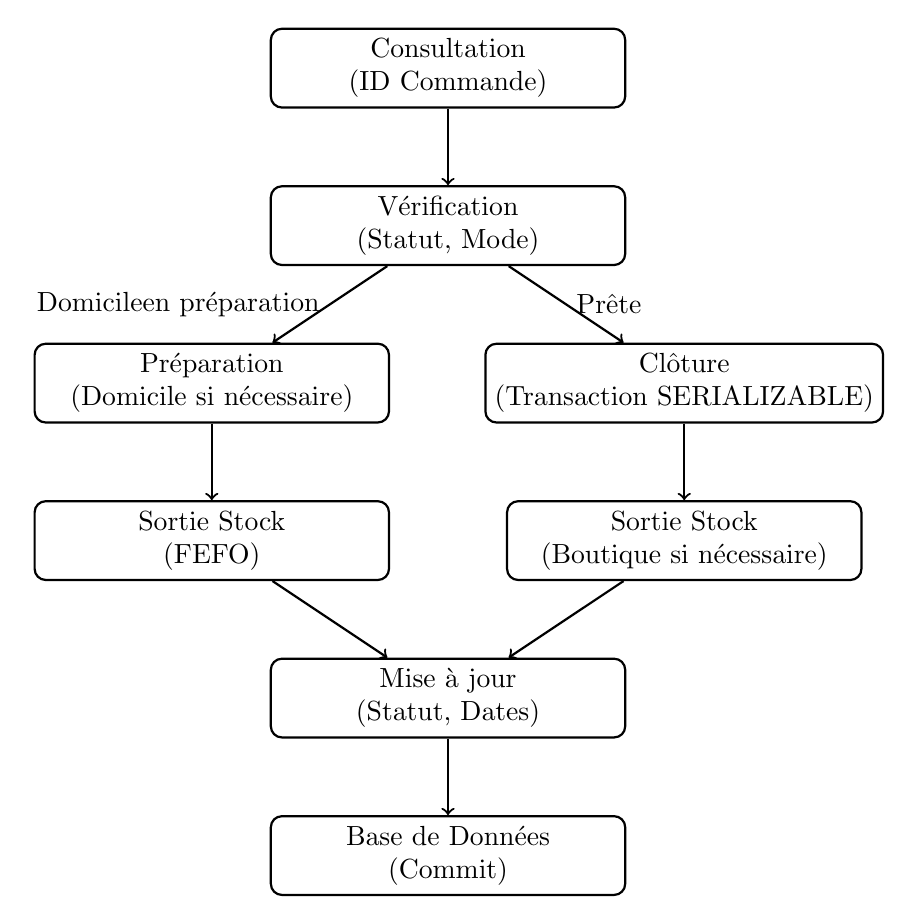
\begin{tikzpicture}[
    node distance=2cm,
    box/.style={
        rectangle,
        draw,
        rounded corners,
        thick,
        minimum width=4.5cm,
        minimum height=1cm,
        align=center
    },
    arrow/.style={->, thick}
]

% Nodes
\node[box] (consult) {Consultation\\(ID Commande)};

\node[box, below of=consult] (check) {Vérification\\(Statut, Mode)};

\node[box, below of=check, xshift=-3cm] (prep) {Préparation\\(Domicile si nécessaire)};

\node[box, below of=check, xshift=3cm] (clot) {Clôture\\(Transaction SERIALIZABLE)};

\node[box, below of=prep] (stock1) {Sortie Stock\\(FEFO)};

\node[box, below of=clot] (stock2) {Sortie Stock\\(Boutique si nécessaire)};

\node[box, below of=stock1, xshift=3cm] (final) {Mise à jour\\(Statut, Dates)};

\node[box, below of=final] (bdd) {Base de Données\\(Commit)};

% Arrows
\draw[arrow] (consult) -- (check);
\draw[arrow] (check) -- node[left]{Domicile\\en préparation} (prep);
\draw[arrow] (check) -- node[right]{Prête} (clot);
\draw[arrow] (prep) -- (stock1);
\draw[arrow] (clot) -- (stock2);
\draw[arrow] (stock1) -- (final);
\draw[arrow] (stock2) -- (final);
\draw[arrow] (final) -- (bdd);

\end{tikzpicture}
\caption{Processus de clôture d'une commande : de la consultation à la finalisation.}
\end{figure}

